\documentclass{standalone}
\usepackage{tikz}
\usetikzlibrary{patterns}
\usetikzlibrary{positioning}
\usetikzlibrary{patterns, positioning}
\usetikzlibrary{shapes.misc}
\usepackage[outline]{contour}
\contourlength{1.5pt} 
\usepackage[sfdefault]{ClearSans}

\begin{document}
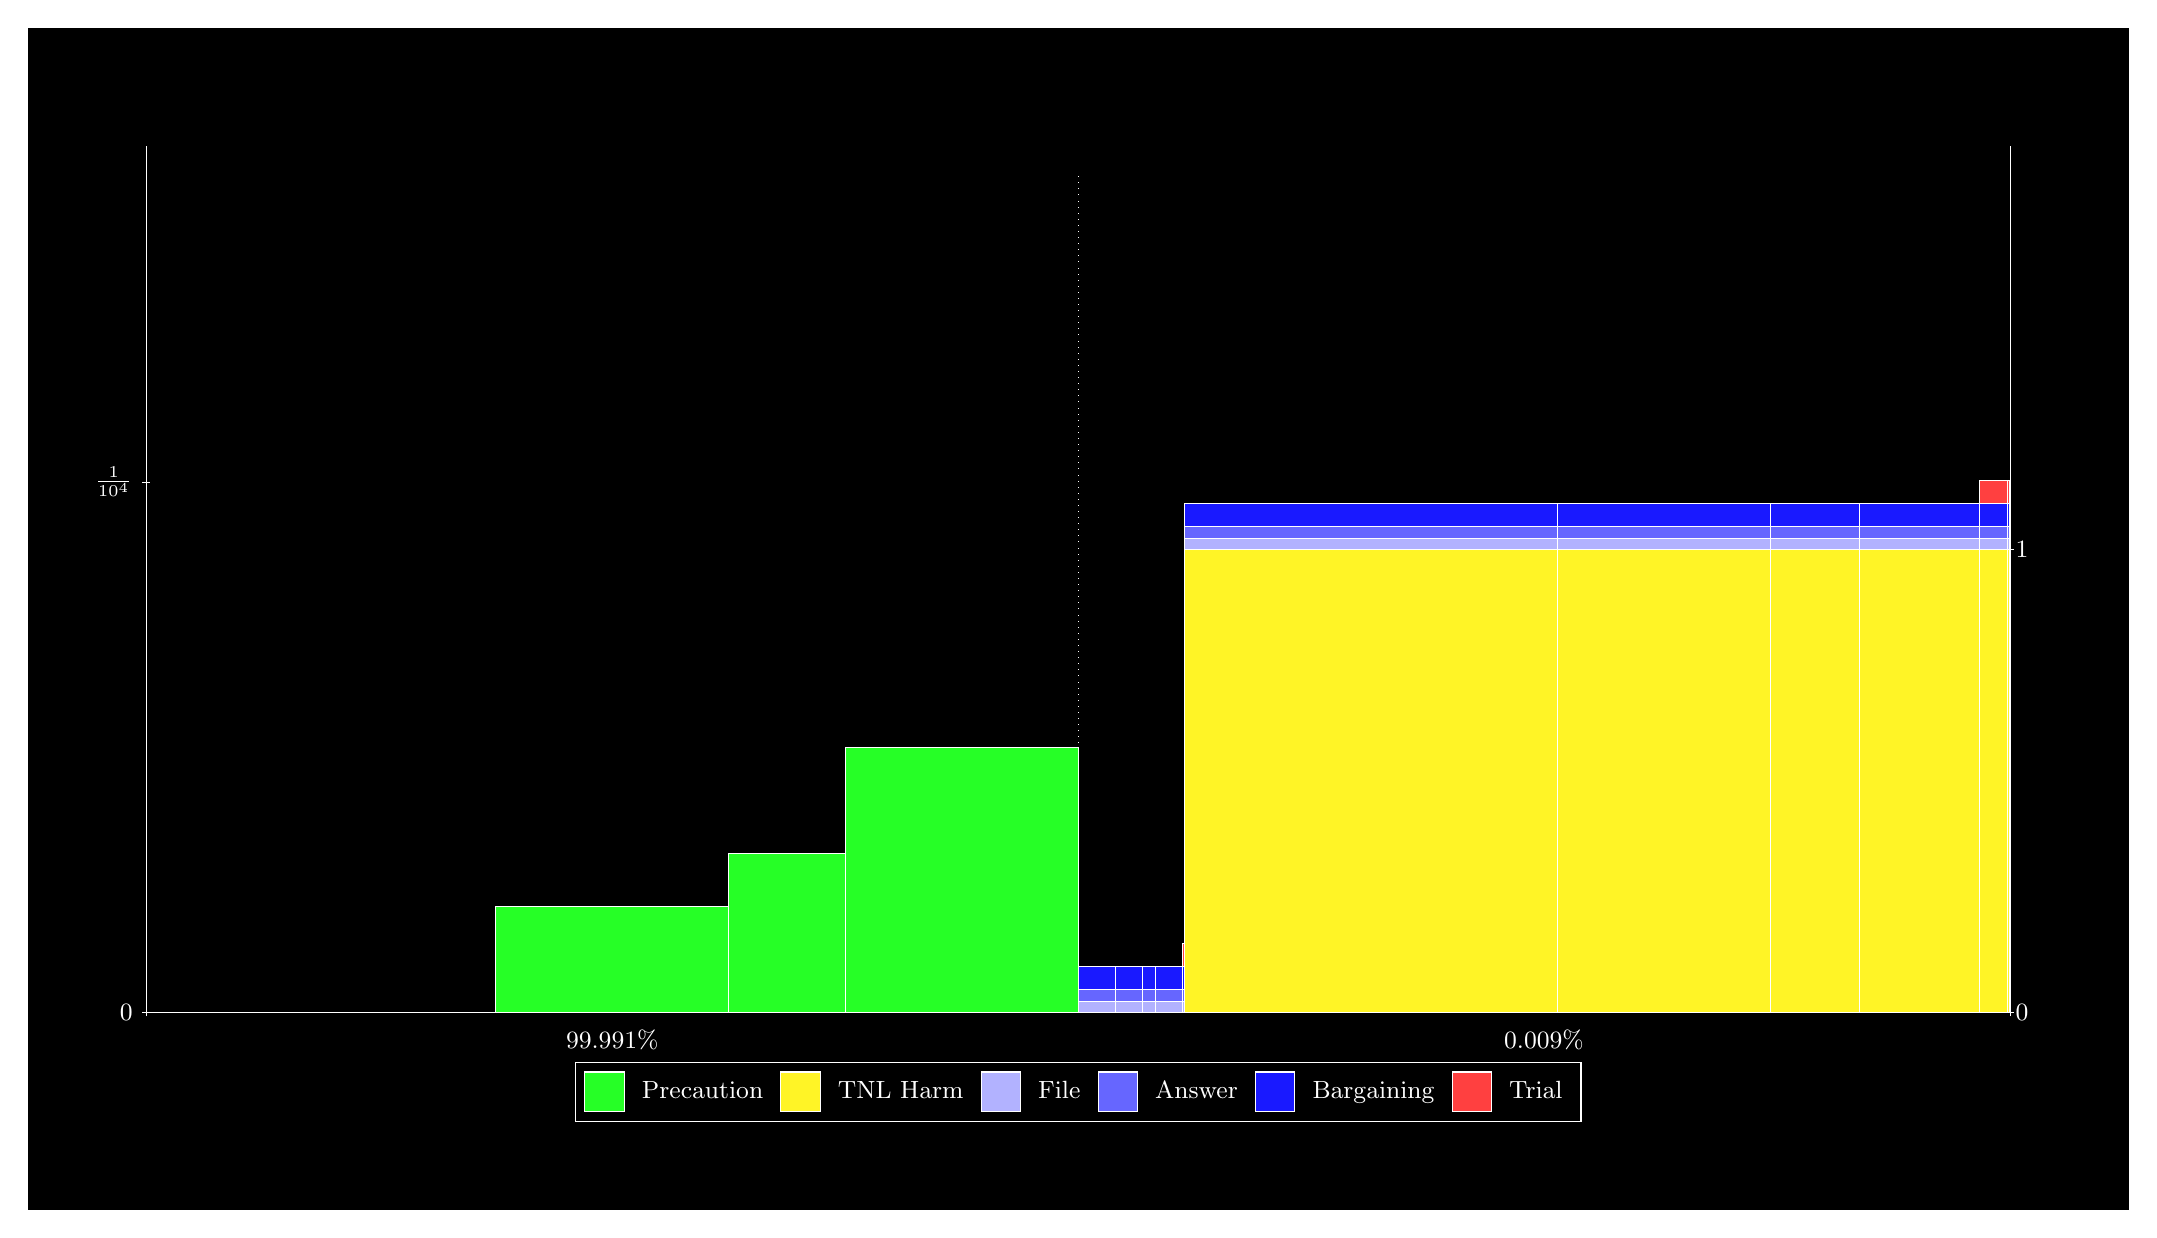
\begin{tikzpicture}
\draw[fill=black] (0,0) rectangle (26.667,15);
\draw[fill=green!85,draw=white,very thin] (5.9374,2.5) rectangle (8.8957,3.8478);
\draw[fill=green!85,draw=white,very thin] (8.8957,2.5) rectangle (10.375,4.5217);
\draw[fill=green!85,draw=white,very thin] (10.375,2.5) rectangle (13.333,5.8694);
\draw[fill=blue!30,draw=white,very thin] (13.333,2.5) rectangle (13.806,2.647);
\draw[fill=blue!60,draw=white,very thin] (13.333,2.647) rectangle (13.806,2.794);
\draw[fill=blue!90,draw=white,very thin] (13.333,2.794) rectangle (13.806,3.0879);
\draw[fill=green!85,draw=white,very thin] (13.806,2.5) rectangle (14.144,2.5001);
\draw[fill=blue!30,draw=white,very thin] (13.806,2.5001) rectangle (14.144,2.6471);
\draw[fill=blue!60,draw=white,very thin] (13.806,2.6471) rectangle (14.144,2.7941);
\draw[fill=blue!90,draw=white,very thin] (13.806,2.7941) rectangle (14.144,3.088);
\draw[fill=green!85,draw=white,very thin] (14.144,2.5) rectangle (14.311,2.5002);
\draw[fill=blue!30,draw=white,very thin] (14.144,2.5002) rectangle (14.311,2.6472);
\draw[fill=blue!60,draw=white,very thin] (14.144,2.6472) rectangle (14.311,2.7941);
\draw[fill=blue!90,draw=white,very thin] (14.144,2.7941) rectangle (14.311,3.0881);
\draw[fill=green!85,draw=white,very thin] (14.311,2.5) rectangle (14.651,2.5003);
\draw[fill=blue!30,draw=white,very thin] (14.311,2.5003) rectangle (14.651,2.6473);
\draw[fill=blue!60,draw=white,very thin] (14.311,2.6473) rectangle (14.651,2.7942);
\draw[fill=blue!90,draw=white,very thin] (14.311,2.7942) rectangle (14.651,3.0882);
\draw[fill=blue!30,draw=white,very thin] (14.651,2.5) rectangle (14.686,2.647);
\draw[fill=blue!60,draw=white,very thin] (14.651,2.647) rectangle (14.686,2.794);
\draw[fill=blue!90,draw=white,very thin] (14.651,2.794) rectangle (14.686,3.0879);
\draw[fill=red!75,draw=white,very thin] (14.651,3.0879) rectangle (14.686,3.3819);
\draw[fill=yellow!85,draw=white,very thin] (14.686,2.5) rectangle (19.417,8.379);
\draw[fill=blue!30,draw=white,very thin] (14.686,8.379) rectangle (19.417,8.526);
\draw[fill=blue!60,draw=white,very thin] (14.686,8.526) rectangle (19.417,8.673);
\draw[fill=blue!90,draw=white,very thin] (14.686,8.673) rectangle (19.417,8.9669);
\draw[fill=green!85,draw=white,very thin] (19.417,2.5) rectangle (22.124,2.5001);
\draw[fill=yellow!85,draw=white,very thin] (19.417,2.5001) rectangle (22.124,8.3791);
\draw[fill=blue!30,draw=white,very thin] (19.417,8.3791) rectangle (22.124,8.5261);
\draw[fill=blue!60,draw=white,very thin] (19.417,8.5261) rectangle (22.124,8.6731);
\draw[fill=blue!90,draw=white,very thin] (19.417,8.6731) rectangle (22.124,8.967);
\draw[fill=green!85,draw=white,very thin] (22.124,2.5) rectangle (23.255,2.5002);
\draw[fill=yellow!85,draw=white,very thin] (22.124,2.5002) rectangle (23.255,8.3792);
\draw[fill=blue!30,draw=white,very thin] (22.124,8.3792) rectangle (23.255,8.5262);
\draw[fill=blue!60,draw=white,very thin] (22.124,8.5262) rectangle (23.255,8.6732);
\draw[fill=blue!90,draw=white,very thin] (22.124,8.6732) rectangle (23.255,8.9671);
\draw[fill=green!85,draw=white,very thin] (23.255,2.5) rectangle (24.783,2.5003);
\draw[fill=yellow!85,draw=white,very thin] (23.255,2.5003) rectangle (24.783,8.3793);
\draw[fill=blue!30,draw=white,very thin] (23.255,8.3793) rectangle (24.783,8.5263);
\draw[fill=blue!60,draw=white,very thin] (23.255,8.5263) rectangle (24.783,8.6733);
\draw[fill=blue!90,draw=white,very thin] (23.255,8.6733) rectangle (24.783,8.9672);
\draw[fill=yellow!85,draw=white,very thin] (24.783,2.5) rectangle (25.139,8.379);
\draw[fill=blue!30,draw=white,very thin] (24.783,8.379) rectangle (25.139,8.526);
\draw[fill=blue!60,draw=white,very thin] (24.783,8.526) rectangle (25.139,8.673);
\draw[fill=blue!90,draw=white,very thin] (24.783,8.673) rectangle (25.139,8.9669);
\draw[fill=red!75,draw=white,very thin] (24.783,8.9669) rectangle (25.139,9.2609);
\draw[fill=green!85,draw=white,very thin] (25.139,2.5) rectangle (25.154,2.5001);
\draw[fill=yellow!85,draw=white,very thin] (25.139,2.5001) rectangle (25.154,8.3791);
\draw[fill=blue!30,draw=white,very thin] (25.139,8.3791) rectangle (25.154,8.5261);
\draw[fill=blue!60,draw=white,very thin] (25.139,8.5261) rectangle (25.154,8.6731);
\draw[fill=blue!90,draw=white,very thin] (25.139,8.6731) rectangle (25.154,8.967);
\draw[fill=red!75,draw=white,very thin] (25.139,8.967) rectangle (25.154,9.261);
\draw[fill=green!85,draw=white,very thin] (25.154,2.5) rectangle (25.167,2.5002);
\draw[fill=yellow!85,draw=white,very thin] (25.154,2.5002) rectangle (25.167,8.3792);
\draw[fill=blue!30,draw=white,very thin] (25.154,8.3792) rectangle (25.167,8.5262);
\draw[fill=blue!60,draw=white,very thin] (25.154,8.5262) rectangle (25.167,8.6732);
\draw[fill=blue!90,draw=white,very thin] (25.154,8.6732) rectangle (25.167,8.9671);
\draw[fill=red!75,draw=white,very thin] (25.154,8.9671) rectangle (25.167,9.2611);
\draw[white,very thin] (1.5,2.5) -- (1.5,13.5);
\draw[white,very thin] (1.45,2.5) -- (1.55,2.5);
\node[font=\small,text=white, anchor=east] at (1.45, 2.5) {0};
\draw[white,very thin] (1.45,9.2389) -- (1.55,9.2389);
\node[font=\small,text=white, anchor=east] at (1.45, 9.2389) {$\frac{1}{10^{4}}$};

\draw[white,dotted,very thin] (13.333,2.83) -- (13.333,13.17);
\draw[white,very thin] (25.167,2.5) -- (25.167,13.5);
\draw[white,very thin] (25.117,2.5) -- (25.217,2.5);
\node[font=\small,text=white, anchor=west] at (25.117, 2.5) {0};
\draw[white,very thin] (25.117,8.379) -- (25.217,8.379);
\node[font=\small,text=white, anchor=west] at (25.117, 8.379) {1};

\draw[white,very thin] (1.5,2.5) -- (25.167,2.5);
\draw[white,very thin] (1.5,2.45) -- (1.5,2.55);
\node[font=\small,text=white, anchor=north] at (1.5, 2.45) {};
\draw[white,very thin] (25.167,2.45) -- (25.167,2.55);
\node[font=\small,text=white, anchor=north] at (25.167, 2.45) {};

\node[font=\small,text=white,anchor=south] at (7.4167, 1.9) {99.991\%};
\node[font=\small,text=white,anchor=south] at (19.25, 1.9) {0.009\%};
\draw (13.3333,2.5) node (B) {};
\begin{scope}[align=center]
\matrix[scale=0.5,draw=white,below=0.5cm of B,nodes={draw},column sep=0.1cm]{
\node[rectangle,draw,minimum width=0.5cm,minimum height=0.5cm,fill=green!85]{}; & \node[draw=none,font=\small,text=white]{Precaution}; &
\node[rectangle,draw,minimum width=0.5cm,minimum height=0.5cm,fill=yellow!85]{}; & \node[draw=none,font=\small,text=white]{TNL Harm}; &
\node[rectangle,draw,minimum width=0.5cm,minimum height=0.5cm,fill=blue!30]{}; & \node[draw=none,font=\small,text=white]{File}; &
\node[rectangle,draw,minimum width=0.5cm,minimum height=0.5cm,fill=blue!60]{}; & \node[draw=none,font=\small,text=white]{Answer}; &
\node[rectangle,draw,minimum width=0.5cm,minimum height=0.5cm,fill=blue!90]{}; & \node[draw=none,font=\small,text=white]{Bargaining}; &
\node[rectangle,draw,minimum width=0.5cm,minimum height=0.5cm,fill=red!75]{}; & \node[draw=none,font=\small,text=white]{Trial}; \\\\
};\end{scope}

\end{tikzpicture}
\end{document}